\section{Introduction}
% Dennard Scaling making energy essential.  Architects address energy
% by making more complicated processors which expose resources to
% software management.  For a wide range of applications, need to meet
% performance goals with minimal energy.
Large classes of computing systems---from embedded to cloud---must
deliver reliable performance while minimizing energy to prolong
battery life or lower operating costs.  To address these conflicting
requirements, hardware architects expose diverse, heterogeneous
resources with a wide array of performance and energy tradeoffs.
Software must allocate these resources to guarantee performance
requirements are met with minimal energy.


% Difficulties of meeting performance with minimal energy. (1)
% complexity---heterogeneous resources---and (2) dynamics---adjust to
% unforeseen changes in workload and environment.
There are two primary difficulties in determining how to allocate
heterogeneous resources.  The first is \emph{complexity}: resources
interact in intricate ways, leading to non-convex optimization spaces.
The second is \emph{dynamics}: perfor\-mance requirements must be met
despite unpredictable disturbances; \eg{} program phases or changes in
operating environment.  Prior work addresses each of these
difficulties individually.

% Prior approaches addressed each of these difficulties individually.
% ML---can handle complexity.  ML advantages: can handle
% non-convexity, avoid local optima, get to true optimal solution. ML
% disadvantages: advanced techniques are expensive and no notion of
% dynamics.  Control---handles dynamics.  Control advantages: formally
% analyzable guarantees despite dynamics.  Control disadvantages:
% relies on good models---no local optima, bounded error.
Machine learning handles complex modern processors, predicting an
application's performance and power as a function of resource
configurations
\cite{reddiHPCA2013,dubach2010,Bitirgen2008,Ipek,Koala,LEO,Flicker,Ponamarev,Paragon}.
These predictions, however, are not useful if the environment changes
dynamically; \eg{} a second application enters the system.  Control
theoretic approaches dynamically adjust resource usage based on the
difference between measured and expected performance
\cite{Steere99,grace,Hellerstein2004a,Chen2011,POET,ControlWare,Agilos,grace2,JouleGuard}.
Control provides formal guarantees that it will meet the performance
goal in dynamic environments, but these guarantees are based on known
relationships between resources and performance.  If the relationships
are not known or there is significant error between the expected and
actual behavior, the controller will fail to deliver the required
performance.

% Want to combine learning and control to address both difficulties
% simultaneously.
%Intuitively, combining learning and control should produce predictable
%behavior in complex, dynamic systems.  There are, however, two major
%challenges to implementing the combination:
Intuitively, combining learning and control should produce predictable
performance in complex, dynamic systems.  Such a combination, however,
must address two major challenges:
\begin{itemize}[leftmargin=1.5em]
\item Dividing the resource allocation problem into sub-tasks that
  suit learning and control's different strengths.
\item Defining abstractions that efficiently combine sub-task solutions,
  while maintaining performance guarantees.
\end{itemize}

We address the first challenge by splitting resource allocation into
two sub-tasks.  The first is learning \emph{speedup}---instead of
absolute performance---so that all unpredictable external interference
is viewed as a change to a \emph{baseline} performance and the
relative speedup is independent of these changes.  Learning is
well-suited to predicting speedups as a function of resource usage and
finding Pareto-optimal tradeoffs in speedup and energy.  The second
sub-task is controlling speedup dynamically based on the difference
between measured and desired performance.  Once the learner has found
Pareto-optimal tradeoffs the problem is convex and well-suited to
adaptive control solutions which guarantee the required speedup even in
dynamic environments.
%Even if the measured performance
%is substantially changed due to external disturbances, the controller
%accounts for these dynamics.

We address the second challenge by defining an interface between
learning and control that maintains control's formal guarantees.  This
interface consists of two parts.  The first is a \emph{performance
  hash table} (PHT) that stores the learned relationship between
configurations and speedup.  The PHT allows the controller to find the
resource allocation that meets a desired speedup with minimal energy
and requires only constant time---$O(1)$---to access.  The second part
of the interface is the learned variance.  Knowing this value, the
controller can adjust itself to maintain formal convergence guarantees
even though the speedup is predicted by a noisy learning mechanism,
rather than directly measured---as it would be in traditional control
design.

\PUNT{Using the ratio of minimum and maximum speedup and the learned
  variance, the controller dynamically sets its error tolerance
  (specifically, it sets the \emph{pole} of its characteristic
  equation).  Communicating the learned variance allows the controller
  to maintain formal convergence guarantees even though speedup is
  predicted by a noisy learning mechanism, rather than directly
  measured as in traditional control design.}


\PUNT{ Intuitively, the combination of learning and control should
  produce predictable behavior in complex, dynamic systems.  The
  combination, however, incurs two major challenges:
  \begin{itemize}[leftmargin=1em]
  \item Dividing the resource allocation problem into sub-tasks that
    suit learning and control's different strengths.
  \item Defining an interface that efficiently combines sub-task
    solutions so that they coordinate well with each other.
  \end{itemize}


  We address the first challenge by adding a layer of indirection. The
  learner learns relative performance (speed-up)---instead of absolute
  performance---so that all unpredictable external interference can be
  viewed as a change to a \emph{baseline} performance and the relative
  speedup is independent of these changes. These speedups are then fed
  into the controller which can use this information to operate
  dynamically. The controller does not need to know the explicit
  mapping between resource configuration and performance but it only
  needs to know the relative ordering between those configurations.


  We address the first challenge by splitting resource allocation into
  two sub-tasks.  The first is learning speedup---instead of absolute
  performance---so that all unpredictable external interference can be
  viewed as a change to a \emph{baseline} performance and the relative
  speedup is independent of these changes.  Learning is well-suited to
  predicting speedups as a function of resource usage and separating
  globally optimal resource configurations from locally optimal ones.

  The second sub-task controlling speedup dynamically based on the
  difference between measured and desired performance.  Once the
  learner has removed locally optimal solutions, the problem is convex
  and well-suited to adaptive control solutions which can deliver
  required speedup even in dynamic environments.
  % Even if the measured performance is substantially changed due to
  % external disturbances, the controller accounts for these dynamics.

  We address the second challenge by defining an interface between
  learning and control that maintains control's formal guarantees.
  This interface consists of two parts.  The first is a
  \emph{performance hash table} (PHT) that stores the learned
  relationship between configurations and speedup.  The PHT allows the
  controller to find the resource allocation that meets a desired
  speedup with minimal energy and requires only constant
  time---$O(1)$---to access.  The second part of the interface is the
  learned variance.  Knowing this value, the controller can adjust
  itself to maintain formal convergence guarantees even though the
  speedup is predicted by a noisy learning mechanism, rather than
  directly measured---as it would be in traditional control
  design.\PUNT{Using the ratio of minimum and maximum speedup and the
    learned variance, the controller dynamically sets its error
    tolerance (specifically, it sets the \emph{pole} of its
    characteristic equation).  Communicating the learned variance
    allows the controller to maintain formal convergence guarantees
    even though speedup is predicted by a noisy learning mechanism,
    rather than directly measured as in traditional control design.}
}

We propose \SYSTEM{}\footnote{\textbf{C}ontrol \textbf{A}nd
  \textbf{L}earning for \textbf{O}ptimal \textbf{R}esource
  \textbf{E}nergy \textbf{E}fficiency} a general methodology allowing
different learning techniques to be paired with a controller.
\SYSTEM{} tunes its internal parameters automatically; \ie{} \emph{it
  requires no user-level inputs other than performance requirements}.
% Implement CALOREE.  Test against state of the art learning and
% self-tuning control systems.  We find that:
We evaluate \SYSTEM{} by implementing the learners on an x86 server
and the controller on heterogeneous ARM big.LITTLE devices.  We
compare to state-of-the-art learning (including polynomial regression
\cite{Koala,dubach2010}, the Netflix algorithm \cite{netflix,Paragon},
and a hierarchical Bayesian model \cite{LEO}) and control (including
proportional-integral-derivative \cite{Hellerstein2004a} and adaptive,
or self-tuning \cite{HandbookControl}) techniques.  We set performance
goals for benchmark applications and measure both the percentage of
time the requirements are violated and the energy.  We test both
\emph{single-app}---where an application runs alone---and
\emph{multi-app} environments---where background applications
unpredictably enter the system and compete for resources.  \SYSTEM{}
achieves the:
\begin{itemize}[leftmargin=1em]
\item \textit{Most reliable performance:}
  \begin{itemize}[leftmargin=1em]
  \item In the \emph{single-app} case, the best prior technique misses
    12\% of deadlines on average, while \SYSTEM{} misses only 5\% on
    average---reducing deadline misses by more than 58\% compared to
    prior approaches.
  \item In the \emph{multi-app} case, the best prior approach averages
    24\% deadline misses, but \SYSTEM{} misses just 6\% of
    deadlines---a huge improvement over prior work.
  \end{itemize}
\item \textit{Best energy savings:} We compare to an \emph{oracle}
  with a perfect model of the application, system, and future events.
  \begin{itemize}[leftmargin=1em]
  \item In the \emph{single-app} case, the best prior approach
    averages 12\% more energy consumption than the oracle, but
    \SYSTEM{} consumes only 5\% more.
  \item In the \emph{multi-app} case, the best prior approach averages
    16\% more energy than the oracle, while \SYSTEM{} consumes just
    9\% more.
  \end{itemize}
\end{itemize}

% Key contributions.
% Contributions, but I decided against bulleted llist for thsi paper
In summary, \emph{\SYSTEM{} is the first work to combine learning and
  control to ensure application performance---both formally and
  empirically---without requiring prior knowledge of the controlled
  application.}  \SYSTEM{}'s contributions are:
\begin{itemize}[leftmargin=1em]
\item Separation of resource management into (1) \emph{learning}
  complicated resource interactions and (2) \emph{controlling}
  speedup.
\item A generalized control design for use with multiple learners.
\item A data structure for constant time access to learned models.
\item Identification of variance as the key to guaranteeing
  performance using learned---rather than measured---data.
\item Demonstration of practical benefits using mobile/embedded
  processors as a case study.
\end{itemize}

%\begin{wrapfigure}{r}{0.5\columnwidth}
\begin{figure}
\centering
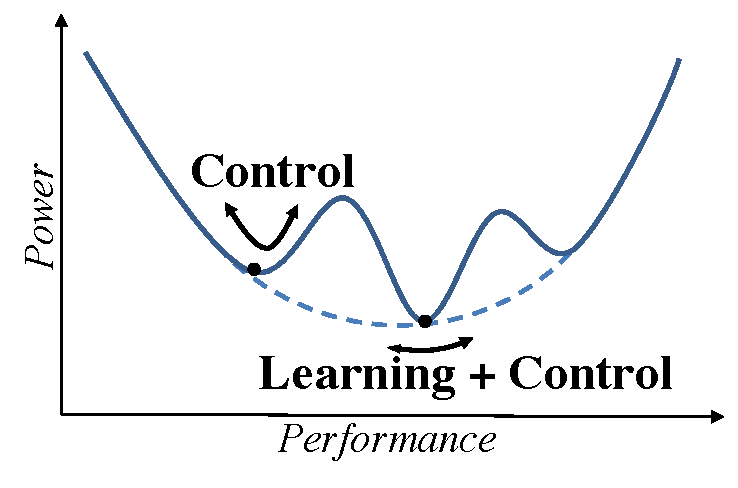
\includegraphics[width=.5\columnwidth]{figures/learning_control_doodle.pdf}
\caption{Learning makes controller's domain smooth.}
\label{fig:learning-control-doodle}
\end{figure}
%\end{wrapfigure}
% Formal analysis of \SYSTEM{} demonstrates convergence
% despite noisy inputs and shows how to integrate learned variance into
% control theoretic guarantees.  We demonstrate the practical benefits
% of these contributions for mobile/embedded processors, finding
% \SYSTEM{} provides much more reliable performance and lower energy
% than learning or control solutions alone.